\chapter{Estado del Arte}

\section{Información previa a considerar}

Para entrar de lleno en la tema, es necesario conocer de antemano varios aspectos básicos de la biología.

\subsection{Biomoléculas}

Cada vez que se habla de la biología, este concepto se relaciona directamente con la ciencia que estudia a los seres vivos. Ahora bien, las estructuras o compuestos que constituyen una parte esencial de los seres vivos son conocidas como \textbf{biomoléculas}. Estas biomoléculas están principalmente constituidas por elementos químicos como el carbono (C), hidrógeno (H), oxígeno (O), nitrógeno (N), fósforo (P) y azufre (S) \cite{biomolecula} y se pueden clasificar en biomoléculas inorgánicas, que se encuentran tanto en seres vivos como en los cuerpos inertes, no obstante son imprescindibles para la vida; y las biomoléculas orgánicas, que son sintetizadas por los seres vivos y tienen una estructura con base en carbono. Estas biomoléculas orgánicas se pueden separar en 4 grandes grupos:
\begin{enumerate}
\item Glúcidos (hidratos de carbono o carbohidratos): son la fuente de energía primaria que utilizan los seres vivos para realizar sus funciones vitales. Los ejemplos más conocidos son la glucosa, el almidón y el glucógeno.
\item Lípidos: conforman el principal almacén de energía de los animales y desempeñan funciones reguladores de enzimas y hormonas.
\item Ácidos nucleicos: El ácido desoxirribonucleico y el ácido ribonucleico, mayormente conocidos como ADN (DNA) y ARN (RNA y sus derivados) desarrollan posiblemente la función más importante para la vida: contener, de manera codificada, las instrucciones necesarias para el desarrollo y funcionamiento de la célula. El ADN tiene la capacidad de replicarse, transmitiendo así dichas instrucciones a las células hijas que heredarán la información.
\item Proteínas: poseen la mayor diversidad de funciones que realizan en los seres vivos; prácticamente todos los procesos biológicos dependen de su presencia y/o actividad. Son proteínas casi todas las enzimas, catalizadores de reacciones metabólicas, hemoglobina, anticuerpos, entre otros. Su unidad base es el {\it{aminoácido}}, por el cual se van formando los péptidos según la cantidad de unidades bases enlazadas.
\end{enumerate}

Dentro de estas biomoléculas, el análisis detallado de los carbohidratos y los lípidos depende en demasía de su estructura química (elementos químicos asociados y tipo de enlaces entre ellos), por lo mismo es una materia más ligada a los químicos (ver Figura 1.1). 

\begin{figure}[H] 

\begin{subfigure}{0.5\textwidth}
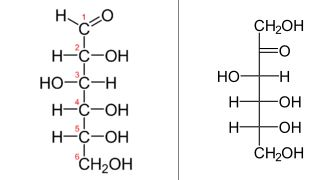
\includegraphics[width=0.9\linewidth, height=5cm]{./images/glucidoejemplos} 
\caption{Glúcidos (glucosa y fructosa)}
\label{fig:subim1}
\end{subfigure}
\begin{subfigure}{0.4\textwidth}
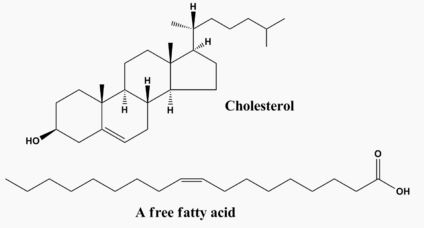
\includegraphics[width=1\linewidth, height=5cm]{./images/lipidosejemplos}
\caption{Lípidos (colesterol y un ácido graso)}
\label{fig:subim2}
\end{subfigure}
 
\caption{Estructura química de los carbohidratos y lípidos.}
\label{fig:image1}
\end{figure}

Sin embargo, el ADN y los polipéptidos poseen unidades base que pueden ser codificadas como letras, por consiguiente pueden ser secuenciados como {\it{cadenas de strings}} y en donde los avances computacionales y la evolución informática toman una importante relevancia (ver Figura 1.2).

\begin{figure}[H]

\begin{subfigure}{0.5\textwidth}
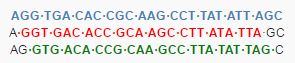
\includegraphics[width=1\linewidth, height=2cm]{./images/adnejemplo}
\caption{Cadena de ADN aleatoria}
\label{fig:subim4}
\end{subfigure}
\begin{subfigure}{0.4\textwidth}
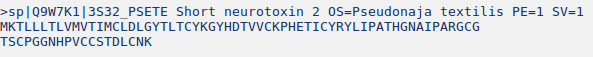
\includegraphics[width=1\linewidth, height=5cm]{./images/cadena} 
\caption{Cadenas $\alpha$ y $\beta$ de hemoglobina bovina}
\label{fig:subim3}
\end{subfigure}
 
\caption{Biomoléculas de ADN y péptidos llevadas a cadenas de strings.}
\label{fig:image2}
\end{figure}

Con respecto a estas 2 últimas estructuras, la diferencia visual más notoria radica en la cantidad de diferentes letras (strings) que las componen, para el ADN son 4 [8] y son denominadas \textbf{bases nitrogenadas} que son las siguientes:

\begin{enumerate}
\item Adenina
\item Timina
\item Citosina
\item Guanina
\end{enumerate}

Para las proteínas, su elemento básico, como ya se mencionó anteriormente es el \textbf{aminoácido}, pero ahora se adentrará en más detalle sobre esta molécula.

\subsection{Aminoácidos}

Los aminoácidos tienen diferentes funciones en el organismo \cite{amino} pero ante todo sirven como \textbf{las unidades básicas de los péptidos y de las proteínas.} A nivel orgánico el aminoácido es una molécula compuesta con un grupo amino (-NH2) y un grupo carboxilo (-COOH) y que pueden tener distintas distribuciones. Para el caso de los que componen las proteínas se consideran como alfa-aminoácidos:

\begin{figure}[h]
    \centering
    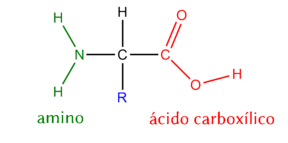
\includegraphics[width=0.4\textwidth]{./images/aminoacido}
    \caption{Estructura general de un alfa-aminoácido}
    \label{fig:image3}
\end{figure}

En la imagen anterior se puede identificar el carbono central (alfa) unido al grupo carboxilo (rojo), grupo amino (verde), un hidrógeno (imagen superior color negro) y el grupo radical (azul) o R. Este grupo radical es el que determina la identidad y las propiedades de cada uno de los diferentes aminoácidos.

El primer aminoácido fue descubierto a principios del siglo XIX, y a partir de ese entonces hasta la actualidad son miles los aminoácidos que han sido descubiertos, pero solo 20 se consideran como los componentes esenciales para las proteínas (y los que se considerarán como parte de esta memoria) que se presentarán a continuación en conjunto con su respectiva abreviación utilizada en las cadenas de proteínas de los archivos FASTA:

\begin{enumerate}
\item Alanina - A
\item Cisteína - C
\item Ácido aspártico - D
\item Ácido glutámico - E
\item Fenilalalina - F
\item Glicina - G
\item Histidina - H
\item Isoleucina - I
\item Lisina - K
\item Leucina - L
\item Metionina - M
\item Aspargarina - N
\item Prolina - P
\item Glutamina - Q
\item Arginina - R
\item Serina - S
\item Treonina - T
\item Valina - V
\item Triptófano - W
\item Tirosina - Y
\end{enumerate}

Existen otras abreviaturas en las cadenas como B, X o J, pero para el alcance de esta memoria no serán considerados como objeto de estudio y análisis posterior.

A partir de este pequeño elemento se forman las macromoléculas que se identifican según la cantidad de aminoácidos (a partir de ahora se mencionarán como aa.) que lo compongan:

\begin{table}[H]
\centering
\label{my-label1}
\begin{tabular}{|c|c|}
\hline
Tamaño & \multicolumn{1}{c|}{Tipo de estructura}  \\ \hline
2 aa.     & Dipéptido        \\
3 aa.     & Tripéptido                         \\
Entre 2 y 8 aa.      &      Oligopéptido                             \\
Menos de 100 aa.      &   Péptido       \\
Mayor o igual de 100 aa.   &   Proteína o polipéptido            \\ \hline
\end{tabular}
\caption{Identificación de macromoléculas según cantidad de aminoácidos}
\end{table}

\section{Secuencias de proteínas}

Desde el momento en que se descubrieron los elementos componentes del ADN y las proteínas, se han investigado sobre las posibles combinaciones que se pueden encontrar entre las bases que los conforman y en que cantidad se encuentran. Para el ADN y sus 4 elementos básicos existen millones de seres vivos, parásitos, virus, protozoos y entre otros que se definen por su código genético, por lo cual encontrar los diversos residuos de bases según un determinado tamaño. En el caso puntual para la finalidad de este escrito y según lo mencionado por \cite{zamyatnin1}, es posible estudiar de manera teórica y con fórmulas matemáticas la cantidad máxima de fragmentos que puede formar una proteína. Considerando como base que el número posible de estructuras peptídicas naturales $P$ están compuestas de diferentes residuos de aminoácidos (incluyendo repeticiones en cadenas de aminoácidos) sigue la siguiente fórmula:

\begin{equation}
P=A^{n}
\end{equation}

Donde $A$ es el número de diferentes aminoácidos existentes, y $n$ es la cantidad de aminácidos correspondientes a la estructura estudiada. Por lo mismo y siguiendo esta fórmula (considerando $A=20$) la cantidad de diferentes combinaciones péptidos de tamaño k que se pueden obtener se aprecian en la siguiente tabla:

\begin{table}[H]
\centering
\label{my-label2}
\begin{tabular}{|c|c|}
\hline
Tamaño péptido (k) & \multicolumn{1}{c|}{Combinaciones posibles ($A^{k}$)}  \\ \hline
2 aa.     & 400        \\
3 aa.     & 8000                         \\
4 aa.      &      160000                             \\
5 aa.      &   3200000       \\
10 aa.      &   1.024$\times 10^{13}$       \\
20 aa.      &   1.049$\times 10^{26}$       \\
50 aa.   &     1.126$\times 10^{65}$   \\ \hline
\end{tabular}
\caption{Combinaciones posibles a obtener según el tamaño del péptido}
\end{table}

Según lo observado en esta tabla se identificar que a medida que el valor de k va en aumento, las posibles combinaciones que se pueden obtener de fragmentos de proteínas pueden llegar a tener valores inimaginables para el ser humano corriente; no obstante, no todas estas estructuras existen o son capaces de ser encontradas en la naturaleza \cite{array}, aun así la diversidad de la búsqueda de estos residuos sigue siendo gigantesca, y por ende difícil de solucionar, y este será uno de los problemas que se intentará solucionar en esta memoria.

Ahora bien, para un polipéptido de tamaño $n$ aminoácidos, el máximo número posible de fragmentos de tamaño $k$ que teóricamente se podrían obtener (considerando las posibles repeticiones de fragmentos) es descrita mediante la siguiente expresión:

\begin{equation}
N_{k}^{teorica}=n+k-1
\end{equation}

Por consecuencia, el máximo número posible de fragmentos (incluye posibles repeticiones) que teóricamente se pueden obtener para una molécula de tamaño $n$, partiendo desde $k=2$ (dipéptidos) hasta $k=n-1$, viene dado por:

\begin{equation}
N_{suma}^{teorica}=\sum_{2}^{n-1} \frac{k(k-1)}{2}-1
\end{equation}

Mediante estas fórmulas, se han calculado la cantidad de posibles fragmentos que se pueden obtener en diferentes oligopéptidos y proteínas:

\begin{table}[H]
\centering
\label{my-label3}
\begin{tabular}{|c|l|r|r|}
\hline
Número & \multicolumn{1}{c|}{Oligopéptido/Proteína} & \multicolumn{1}{c|}{$n$} & \multicolumn{1}{c|}{$N_{suma}^{teorica}$} \\ \hline
1      & Encefalina (varios tipos biológicos)       & 5                        & 9                     \\
2      & Bradiquinina (mamíferos)                   & 9                        & 35                    \\
3      & ACTH (humanos)                             & 39                       & 740                   \\
4      & Cadena $\alpha$ hemoglobina (humanos)          & 141                      & 9869                  \\
5      & Cadena $\beta$ hemoglobina (humanos)          & 146                      & 10584                 \\ \hline
\end{tabular}
\caption{Número máximo posible de fragmentos que se pueden formar en 5 proteínas}
\end{table}

Considerando que para un polipéptido de largo $n$ aminoácidos, si este valor de $n$ es muy alto, se puede obtener una cantidad muy alta de fragmentos de dipéptidos, pero muchos de estos dipéptidos se pueden repetir varias veces en la cadena, por lo tanto, cuando se desea obtener {\bf{el máximo número de fragmentos diferentes}} asociado a un valor $k$ determinado, este puede tener un valor muy bajo en comparación con la cantidad total de fragmentos obtenidos. Por medio de las fórmulas descritas anteriormente, se puede obtener el número máximo de diferentes fragmentos (o fragmentos esperables) asociado a un tamaño $k$:

\begin{equation}
N_{k}^{diff}=N_{k}^{teorica}- R_{k}
\end{equation}

Este valor $R_{k}$, se obtiene introduciendo nuevos parámetros $i$ (que es el número de estructuras idénticas para determinado $k$) y $m$ (el número de diferentes estructuras para el determinado $k$):

\begin{equation}
R_{k}=\sum_{1}^{m}(i-1)
\end{equation}

Por lo tanto, el número máximo de fragmentos diferentes que se pueden obtener en una proteína sigue la siguiente fórmula:

\begin{equation}
N_{suma}^{diff}=\Bigg[\sum_{2}^{n-1} \frac{k(k-1)}{2}-1\Bigg]- \sum_{2}^{n-1}\Bigg[\sum_{1}^{m}(i-1)\Bigg]
\end{equation}
\\
Tomando la información de la base de datos de oligopéptidos EROP-Moscow, para mostrar los valores obtenidos con estas fórmulas, se usará como ejemplo la caseína bovina (proteína proveniente de la vaca). Esta proteína se compone de 4 subunidades, $\alpha - s1$, $\alpha -s2$, $\beta$ y $\kappa$. La siguiente tabla muestra las cantidades teóricas y diferentes de fragmentos obtenidos como dipéptidos y sus sumas totales:

\begin{table}[H]
\centering
\label{my-label4}
\begin{tabular}{|c|l|c|c|c|c|c|}
\hline
Número & \multicolumn{1}{c|}{Caseína bovina (subunidad)} & $n$ & $N_{2}^{teorica}$ & \multicolumn{1}{l|}{$N_{2}^{diff}$} & \multicolumn{1}{l|}{$N_{suma}^{teorica}$} & \multicolumn{1}{l|}{$N_{suma}^{diff}$} \\ \hline
1      & $\alpha - s1$                                   & 199 & 198               & 134                                 & 19700                                     & 19621                                  \\
2      & $\alpha - s2$                                   & 207 & 206               & 131                                 & 21320                                     & 21216                                  \\
3      & $\beta$                                         & 209 & 208               & 124                                 & 21735                                     & 21641                                  \\
4      & $\kappa$                                        & 169 & 168               & 118                                 & 14195                                     & 14138                                  \\
5      & $\alpha - s1 + \alpha - s2 + \beta + \kappa$    & 784 & 780               & 260                                 & 76950                                     & 76304                                  \\ \hline
\end{tabular}
\caption{Número máximo posible de fragmentos que se pueden obtener en una proteína de caseína bovina.}
\end{table}

Se puede identificar que para los fragmentos de dipéptidos, la cantidad de diferentes fragmentos es bastante menor que la cantidad total de fragmentos obtenidos para las 4 subunidades, pero aún así la cantidad de fragmentos diferentes totales obtenidos es prácticamente la misma que la cantidad de fragmentos totales sin diferenciar. Esto es notorio ya que si $k$ va en progresivo aumento, el universo combinatorio de posibles fragmentos formados se acorta drásticamente, lo que también favorece a la baja formación de fragmentos que se repiten.\\


\section{Técnicas utilizadas en el problema}

En \cite{searching} se menciona que buscar secuencias de proteínas en un predeterminado archivo (puede ser de texto o .fasta) es una tarea muy compleja, ya que se formaría un escenario similar al buscar una {\textit{aguja en un pajar}} y recorrer millones de secuencias en cada búsqueda no sería lo más convieniente considerando que la cantidad de proteínas que existen el día de hoy son muchas, por consiguiente una herramienta recomendable sería preprocesar la base de datos de proteínas con alguna técnica conocida o implementada. A continuación se hablará de forma general de algunos algoritmos conocidos que han tratado este problema.

\subsection{Algoritmo de fuerza bruta}

Este es el algoritmo más simple posible, ya que dado un texto de tamaño \textit{n} se revisan todas las posiciones posibles de un patrón de tamaño \textit{k < n} desde el comienzo hasta el final del texto (izquierda a derecha). Para el caso puntual de los archivos .fasta de las proteínas es necesario extraer únicamente las cadenas de secuencias respectivas y adjuntarlas línea a línea (de esa forma es más fácil trabajarlas). Luego, y siguiendo la presunción matemática del número máximo de fragmentos de tamaño \textit{k} cada una de las cadenas se revisa desde la posición 0 hasta la posición \textit{n-1} (el valor de \textit{n} varía según el largo de la cadena de cada proteína) yendo de caracter a caracter un total de \textit{n+k-1} veces para cada secuencia:

\subsection{Algoritmos de búsqueda de strings}

Esta clase de algoritmos (en inglés conocidos como \textit{string searching algorithm}) tratan de localizar si uno o varios strings solicitados (que también se llaman patrones) aparecen en un string más largo o simplemente un texto como tal, considerando el alfabeto que por el cual está compuesto el string de destino o texto. En la mayoría de las ocasiones este alfabeto ($\Sigma$) es el que determina el rendimiento de determinado algoritmo (una variación de este alfabeto puede ayudar o perjudicar la eficiencia de un algoritmo en particular), como también el texto a analizar.
Una clasificación básica de estos algoritmos se puede realizar según la cantidad de strings a encontrar:
\begin{enumerate}
\item Algoritmos de búsqueda de un único patrón (\textit{Single pattern algorithms})
\item Algoritmos de búsqueda de múltiples patrones (\textit{Multiple pattern algorithm})
\end{enumerate}

\subsubsection{Algoritmos de búsqueda de un único patrón}
Como lo dice el mismo título, esta clase de algoritmo de búsqueda consiste en encontrar las ocurrencias de un determinado patrón 